\documentclass[a4paper, 12pt]{article}
\usepackage{graphicx}
\usepackage[utf8]{inputenc}
\usepackage{multirow}
%\usepackage{times}
\usepackage{listings}
\usepackage{supertabular}
\usepackage{cite}
\usepackage{amsthm}
\usepackage{tikz}
\newcommand*\circled[1]{\tikz[baseline=(char.base)]{
            \node[shape=circle,draw,inner sep=2pt] (char) {#1};}}
\newcommand{\todo}[1]{\ensuremath{^{\textrm{\tiny{TODO}\normalsize}}}\footnote{\textbf{TODO:}~#1}}

\newcommand{\jcode}[1]{\textnormal{\texttt{#1}}}
\newcommand{\pcode}[1]{\textnormal{\texttt{#1}}}
\newcommand{\pmodule}[1]{\textnormal{\texttt{#1}}}
\newcommand{\rdfterm}[1]{\textnormal{\textsf{#1}}}

\include{helpers}
\usepackage[pdftex,linktocpage]{hyperref}
\hyperbaseurl{https://github.com/}

\begin{document}
\title{Prefetching SPARQL query cacher}
\author{Kjetil Kjernsmo}
%\institute{Department of Informatics,
%Postboks 1080 Blindern,
%0316 Oslo, Norway}

%\email{kjekje@ifi.uio.no}

\maketitle

\section{Introduction}

This chapter describes an effort to create a proxy that can cache the
results of not only SPARQL queries, but also the results of individual
triple patterns. It will asynchronously analyse executed queries, and
may prefetch the results of certain triple patterns into the cache.

The system is in the convergence of the directions described in this
dissertation: It should relieve the remote endpoint of some of the
burden to evaluated the query and it should add to the robustness of the
open Web SPARQL infrastructure. It uses hypermedia to answer individual
triple patterns, based on Triple Pattern Fragments  \cite{ldf1}. The
system can only answer triple patterns, but other than that, supports
SPARQL 1.1 in its entirety. This was made possible to develop quickly
by the efforts put into the query planning in the Attean framework
described in Section~\ref{sec:conpush}. Caching based on RFC7234
\cite{rfc7234} was shown to be of possible use in the survey I
conducted. Finally, it was planned to be evaluated using
Design of Experiments.

Unfortunately, the system has as of this writing insufficient
performance for an evaluation to be meaningful. Nevertheless, it
points out some interesting lessons with varying degrees of
certainty. This chapter will detail the system, show its design and
features and discuss its failures.

Figure~\ref{fig:messaging} illustrates where caches may be in the
Internet infrastructure, as well as HTTP requests and responses in a
typical deployment scenario of the system.

\begin{figure}
\begin{center}
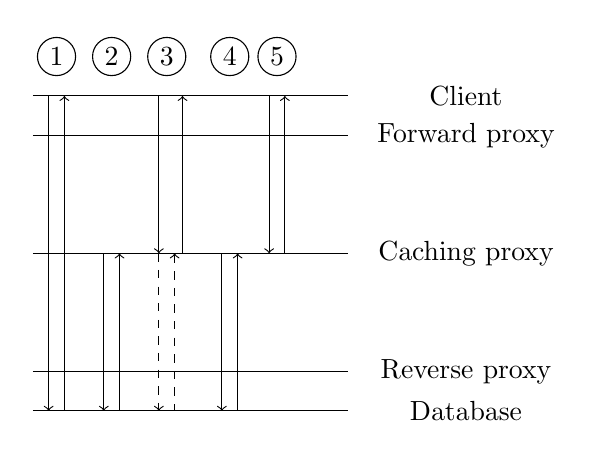
\begin{tikzpicture}
\draw (0,0) --(4,0);
\node at (5.5,0) { Database };
\draw (0,0.5) --(4,0.5);
\node at (5.5,0.5) { Reverse proxy };
\draw (0,2) --(4,2);
\node at (5.5,2) { Caching proxy };
\draw (0,3.5) --(4,3.5);
\node at (5.5,3.5) { Forward proxy };
\draw (0,4) --(4,4);
\node at (5.5,4) { Client };

\draw [->] (0.2,4) --(0.2,0);
\draw [<-] (0.4,4) --(0.4,0);
\node at (0.3,4.5) {\circled{1}};
\draw [->] (0.9,2) --(0.9,0);
\draw [<-] (1.1,2) --(1.1,0);
\node at (1.0,4.5) {\circled{2}};
\draw [->] (1.6,4) --(1.6,2);
\draw [dashed, ->] (1.6,2) --(1.6,0);
\draw [dashed, <-] (1.8,2) --(1.8,0);
\draw [->] (1.9,2) --(1.9,4);
\node at (1.7,4.5) {\circled{3}};
\draw [->] (2.4,2) --(2.4,0);
\draw [<-] (2.6,2) --(2.6,0);
\node at (2.5,4.5) {\circled{4}};
\draw [->] (3,4) --(3,2);
\draw [->] (3.2,2) --(3.2,4);
\node at (3.1,4.5) {\circled{5}};
\end{tikzpicture}
\caption{The possible positions of a cache. A cache may reside at both
  the server side (as a database cache) or client side, or any of the
  intermediate proxies. The arrows illustrate requests (when pointing
  down) and responses (when pointing up) in a deployment scenario for
  when a the query cache considered in this paper is deployed on a
  caching proxy in the Internet infrastructure, see the text for
  details.}\label{fig:messaging}
\end{center}
\end{figure}

The system is based on HTTP, which implies a client-server
architecture. In this architecture, a cache may be present at
conceptually five different levels. First, the client may have its own
cache, which caches only responses made by the client itself. The next
level is known as a forward proxy. They aren't currently very common,
but have in the past often been institutional proxies, or proxies
employed by Internet Service Providers for caching responses that may
be common to many of their users. The next level, generically referred
to as a caching proxy, may be in the Internet
infrastructure. Currently, the most common form of this type of proxy
is known as a Content Delivery Network (CDN). It is very common to
have a reverse proxy near the server. They are often known as a ``Web
Accelerator''. Usually, they will communicate with the server with
HTTP, but it is conceivable that it may use a different protocol, and
may employ detailed knowledge of the hosted data to optimise cache
operations. Finally, the database, in this context a SPARQL Endpoint,
may use conventional database caching techniques. The database cache
and reverse proxy is typically controlled by the data provider.

The present system may be deployed at any of these levels. However,
since the database and the reverse proxy in front of it may have
detailed knowledge of the data, e.g. a complete data profile with
statistics to optimise join order, these levels have much in common
with a conventional database cache, which is extensively discussed in
the literature.

My interest is the case where the caching proxy has no further
knowledge of the data than what is exposed through the SPARQL Endpoint
or hypermedia metadata. In practice, there is very little
information. If the cache is to be shared, then it would typically
reside on the forward proxy, or in a CDN. 

Figure~\ref{fig:messaging} illustrates the case where HTTP messages
are being passed, where the cache is assumed to reside on a
intermediate caching proxy in the Internet, i.e. a CDN. The figure may
be viewed as having time on the $x$-axis, with the arrows pointing
down being requests and the arrows point up being responses. In this
example, the client first makes a request (request \circled{1}), which
is passed through the proxy because it has not yet cached any
responses. The response (response \circled{1}) is then also
transmitted directly from the SPARQL Endpoint at the database back to
the client. The entire response may be cached at the proxy in case it
can be reused in its entirety. However, the main point is that the
request will be analysed by the proxy in parallel to being sent to the
server, and another request \circled{2} for a triple pattern fragment
that the analyser thinks will enable the proxy to assist the server
the best for future requests, is sent. This analysis is discussed in
\todo{ref}. The response \circled{2} is not sent back to the client,
but will enter the cache. Lets say that the analyser was successful
and that the cache can be used to answer request \circled{3}. In that
case, the proxy will send a rewritten query for the rest of the data
it needs to answer the query to the origin server, indicated by the
dashed arrows. This may be a SPARQL query, a TPF request or a
combination thereof, depending on what the planner finds least
expensive. The proxy will then evaluate the entire query and send the
final result back as response \circled{3}. In addition, the analyser
may have identified another Triple Pattern Fragment that it takes as
likely useful for future requests, and sends a request and caches the
response \circled{4}. At some point, it may be able to answer the
entire query using only cached results, as illustrated by request and
response \circled{5}.

\section{Implementation}\label{sec:impl}

The implementation consists of several modules that have been
published to the Comprehensive Perl Archive Network as Free Software,
and most of which have become a part the Free Software ecosystem. To
install the system on the top of a Debian system with only essential
packages requires 146 Debian packages. Running the test suite requires
even more. As such, it builds on the code of hundreds of authors, too
long to enumerate. I shall constrain myself to list the modules that
have code that has been motivated from this study. Modules that have
other primary authors than myself have been started prior to this
present project, but may have substantial contributions from this
project. The Attean framework was started as part of the effort in
Section~\ref{sec:conpush}, but even though it has been developed
further with the requirements that arose from this project and has
contributions from me, the vast majority of the code has been written
my Gregory Todd Williams. The main work in this project has gone into
the module \pmodule{AtteanX::Query::Cache}, where I have authored the vast
majority of the code. The relative difference in authorship can be
further examined by checking the linked Github repositories, or by
using git2prov\footnote{see \url{http://git2prov.org/}} to create RDF
data of the commit history. Table~\ref{tab:modules} shows the modules
that have been influenced or written as part of this project.

\begin{table}
\caption{The modules that enable the query cache}\label{tab:modules}
\begin{tabular}{ | l | p{3cm} | l |}
  \hline
  Module & Authors & Github URL \\ \hline

  \pmodule{AtteanX::Query::Cache} & Kjetil Kjernsmo, Gregory Todd Williams &
  \url{kjetilk/p5-atteanx-query-cache} \\

  \pmodule{AtteanX::Store::SPARQL} & Kjetil Kjernsmo &
  \url{kjetilk/p5-atteanx-store-sparql} \\
  
  \pmodule{AtteanX::Store::LDF} & Kjetil Kjernsmo, Patrick Hochstenbach &
  \url{phochste/AtteanX-Store-LDF} \\

  \pmodule{LWP::UserAgent::CHICaching} & Kjetil Kjernsmo &
  \url{kjetilk/p5-lwp-useragent-chicaching} \\
  
  \pmodule{Attean} & Gregory Todd Williams, Kjetil Kjernsmo &
  \url{kasei/attean} \\

  \pmodule{AtteanX::Endpoint} & Gregory Todd Williams &
  \url{kasei/atteanx-endpoint} \\

  \pmodule{RDF::LDF} &  Patrick Hochstenbach, Gregory Todd Williams, Jakob Voß,
  Kjetil Kjernsmo & \url{phochste/RDF-LDF} \\
  
  \hline
\end{tabular}
\end{table}

The system also depends on modules I have written that is not part of
the project: \pmodule{RDF::LinkedData}, \pmodule{RDF::Generator::Void}, \pmodule{Test::RDF},
\pmodule{URI::NamespaceMap} and \pmodule{RDF::NS::Curated}.

To further understand the roles of the different modules, note the
following: \pmodule{LWP::UserAgent::CHICaching} is a traits-based \cite{traits} implementation of the
majority of RFC7234. \pmodule{AtteanX::Endpoint} is an implementation of the
server side of SPARQL 1.1 Protocol. 

\subsection{The Attean framework}

\subsection{SPARQL protocol client}

The \pmodule{AtteanX::Store::SPARQL} module is a partial SPARQL
Protocol client that implements Attean APIs. The store implementation
itself composes the TripleStore API and implements methods to retrieve
the results of a single triple pattern and exact cardinality for a
given triple pattern, by using an aggregate query. In addition, it can
generate plans for Basic Graph Pattern algebra objects that have more
than one triple pattern. If that is the case, it will return an
instance of the class \pmodule{AtteanX::Plan::SPARQLBGP}, which is
also defined by the module. If it is not the case, the module also has
an implementation of the \pcode{access\_plan} method in a
\pmodule{AtteanX::Query::AccessPlan::SingleQuadBGP} role, that can be
composed by a query planner to provide a single triple pattern
\pmodule{AtteanX::Plan::SPARQLBGP} object. Finally, it also provides a
model implementation that composes the Model and CostPlanner
APIs. This contains a \pcode{cost\_for\_plan} implementation that will
provide a cost for \pmodule{AtteanX::Plan::SPARQLBGP} objects that are
proportional to the number of triple patterns in the plan, but
penalises plans that does not have triple patterns that are connected
through a variable (i.e. will cause a Cartesian join) with a factor
10. See Section~\ref{sec:costheuristics} for details on the cost
heuristics. 

\subsection{Linked Data Fragment client}




\bibliography{management,dataprofiles,federation,dynamicity,hypermedia,specs,webarch,practical,semweb,caching,critisism,data,philosophy,benchmarks,rfc,programming,egne}
\bibliographystyle{plain}

\end{document}
